\documentclass[border=12pt]{standalone}
\usepackage[dvipsnames]{xcolor}
\usepackage{tikz}
\usetikzlibrary{arrows.meta, positioning, calc, shadows, shapes.geometric}

\definecolor{gold}{HTML}{CFB87C}
\definecolor{dkblue}{HTML}{156082}
\definecolor{accent2}{HTML}{E97132}
\definecolor{accent3}{HTML}{196B24}
\definecolor{dkgray}{HTML}{333333}
\definecolor{medgray}{HTML}{888888}
\definecolor{ltgold}{HTML}{F5F0E6}
\definecolor{cardbg}{HTML}{FAFAF7}

\begin{document}
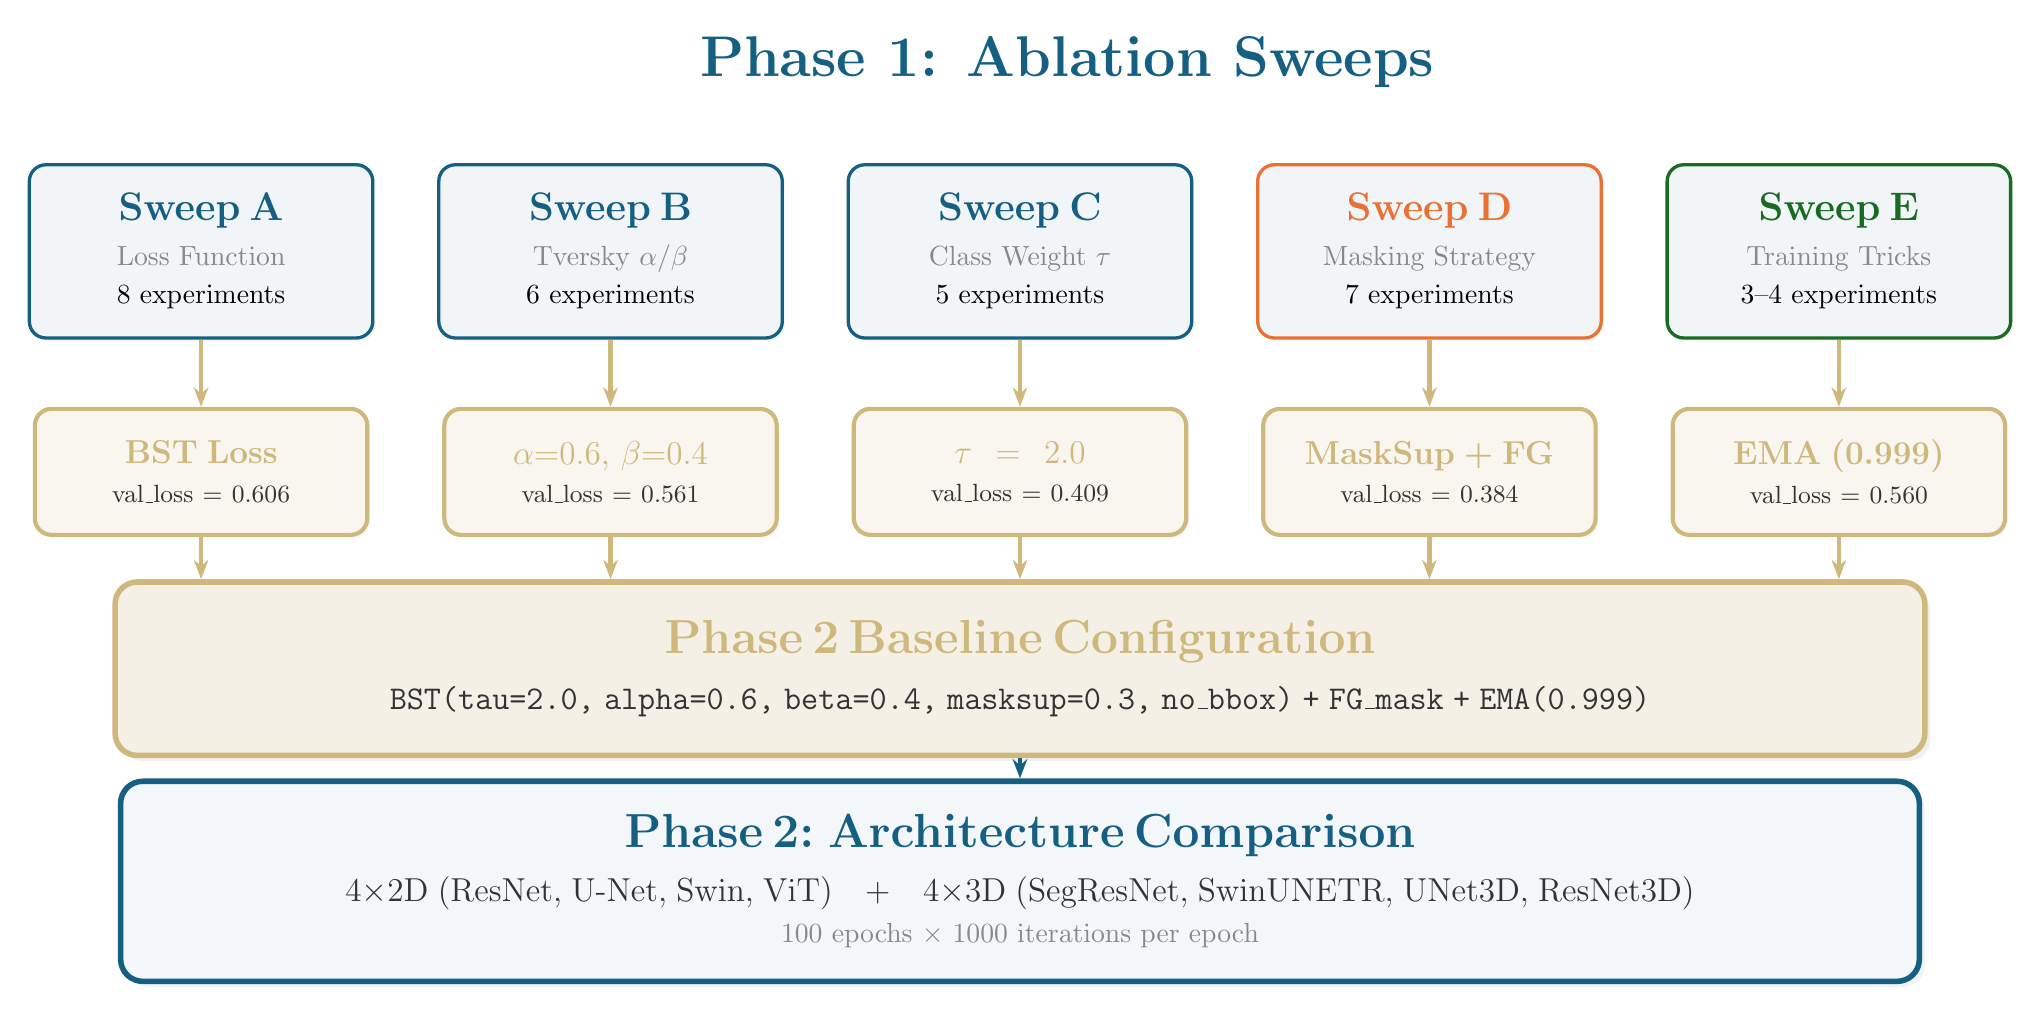
\begin{tikzpicture}[
    node distance=0.5cm and 0.5cm,
    sweep/.style={
        draw=dkblue, fill=dkblue!6, rounded corners=6pt,
        line width=1.2pt, minimum width=4.2cm, minimum height=2.2cm,
        text width=3.8cm, align=center, font=\normalsize, inner sep=8pt,
        drop shadow={shadow xshift=1pt, shadow yshift=-1pt, opacity=0.08}
    },
    winner/.style={
        draw=gold, fill=gold!12, rounded corners=6pt,
        line width=1.5pt, minimum width=4.2cm, minimum height=1.6cm,
        text width=3.8cm, align=center, font=\normalsize, inner sep=6pt,
        drop shadow={shadow xshift=1pt, shadow yshift=-1pt, opacity=0.08}
    },
    compose/.style={
        draw=gold, fill=ltgold, rounded corners=8pt,
        line width=2pt, minimum height=2.2cm,
        text width=22cm, align=center, font=\normalsize, inner sep=14pt,
        drop shadow={shadow xshift=2pt, shadow yshift=-2pt, opacity=0.12}
    },
    phase2box/.style={
        draw=dkblue, fill=dkblue!5, rounded corners=8pt,
        line width=2pt, minimum height=2.0cm,
        text width=22cm, align=center, font=\normalsize, inner sep=12pt,
        drop shadow={shadow xshift=2pt, shadow yshift=-2pt, opacity=0.10}
    },
    garrow/.style={-{Stealth[length=7pt]}, line width=1.5pt, color=gold},
    barrow/.style={-{Stealth[length=7pt]}, line width=1.5pt, color=dkblue},
    >=Stealth
]

% --- Phase 1 title ---
\node[font=\huge\bfseries, color=dkblue] at (11, 8.2) {Phase 1: Ablation Sweeps};

% --- Sweep boxes (row 1) ---
\node[sweep] (sa) at (0, 5.8) {%
    {\Large\bfseries\color{dkblue}Sweep A}\\[4pt]
    {\color{medgray}Loss Function}\\[2pt]
    8 experiments%
};
\node[sweep] at (5.2, 5.8) (sb) {%
    {\Large\bfseries\color{dkblue}Sweep B}\\[4pt]
    {\color{medgray}Tversky $\alpha/\beta$}\\[2pt]
    6 experiments%
};
\node[sweep] at (10.4, 5.8) (sc) {%
    {\Large\bfseries\color{dkblue}Sweep C}\\[4pt]
    {\color{medgray}Class Weight $\tau$}\\[2pt]
    5 experiments%
};
\node[sweep, draw=accent2] at (15.6, 5.8) (sd) {%
    {\Large\bfseries\color{accent2}Sweep D}\\[4pt]
    {\color{medgray}Masking Strategy}\\[2pt]
    7 experiments%
};
\node[sweep, draw=accent3] at (20.8, 5.8) (se) {%
    {\Large\bfseries\color{accent3}Sweep E}\\[4pt]
    {\color{medgray}Training Tricks}\\[2pt]
    3--4 experiments%
};

% --- Winner boxes (row 2) ---
\node[winner] (wa) at (0, 3.0) {%
    {\large\bfseries\color{gold}BST Loss}\\[2pt]
    {\small\color{dkgray}val\_loss = 0.606}%
};
\node[winner] (wb) at (5.2, 3.0) {%
    {\large\bfseries\color{gold}$\alpha{=}0.6,\,\beta{=}0.4$}\\[2pt]
    {\small\color{dkgray}val\_loss = 0.561}%
};
\node[winner] (wc) at (10.4, 3.0) {%
    {\large\bfseries\color{gold}$\tau = 2.0$}\\[2pt]
    {\small\color{dkgray}val\_loss = 0.409}%
};
\node[winner] (wd) at (15.6, 3.0) {%
    {\large\bfseries\color{gold}MaskSup + FG}\\[2pt]
    {\small\color{dkgray}val\_loss = 0.384}%
};
\node[winner] (we) at (20.8, 3.0) {%
    {\large\bfseries\color{gold}EMA (0.999)}\\[2pt]
    {\small\color{dkgray}val\_loss = 0.560}%
};

% --- Sweep -> Winner arrows ---
\foreach \s/\w in {sa/wa, sb/wb, sc/wc, sd/wd, se/we} {
    \draw[garrow] (\s.south) -- (\w.north);
}

% --- Composed config box ---
\node[compose] (config) at (10.4, 0.5) {%
    {\LARGE\bfseries\color{gold}Phase 2 Baseline Configuration}\\[8pt]
    {\large\ttfamily\color{dkgray}%
        BST(tau=2.0,\ alpha=0.6,\ beta=0.4,\ masksup=0.3,\ no\_bbox)\ +\ FG\_mask\ +\ EMA(0.999)}%
};

% --- Winner -> Config arrows (converging) ---
\foreach \w in {wa, wb, wc, wd, we} {
    \draw[garrow] (\w.south) -- (config.north -| \w.south);
}

% --- Phase 2 box ---
\node[phase2box] (p2) at (10.4, -2.2) {%
    {\LARGE\bfseries\color{dkblue}Phase 2: Architecture Comparison}\\[6pt]
    {\large\color{dkgray}%
        4$\times$2D (ResNet, U-Net, Swin, ViT)\quad+\quad4$\times$3D (SegResNet, SwinUNETR, UNet3D, ResNet3D)}\\[3pt]
    {\normalsize\color{medgray}100 epochs $\times$ 1000 iterations per epoch}%
};

\draw[barrow] (config.south) -- (p2.north);

\end{tikzpicture}
\end{document}
